\documentclass[12pt,a4paper,oneside]{book}

	\makeatletter
	\newcommand\thefontsize[1]{{}}
	\makeatother
	\usepackage[utf8]{inputenc}
	\usepackage{enumitem}
	\usepackage{varwidth}
	\usepackage{graphicx}
	\usepackage{caption}
	
\usepackage[top=2.5cm, bottom=3cm, left=2.5cm, right=2.5cm]{geometry}
\usepackage[utf8]{inputenc}
\usepackage[titletoc,title]{appendix}
\usepackage[linewidth=1pt]{mdframed}
\usepackage{framed}
\usepackage{listings}
\usepackage{smartdiagram}
\usepackage{smartdiagram}
\usepackage{varwidth}
\usepackage{amsmath}
\usepackage[linesnumbered,ruled,vlined]{algorithm2e}
\usesmartdiagramlibrary{additions}
\lstdefinestyle{customc}{
	belowcaptionskip=1\baselineskip,
	breaklines=true,
	frame=L,
	xleftmargin=\parindent,
	language=C,
	showstringspaces=false,
	basicstyle=\footnotesize\ttfamily,
	keywordstyle=\bfseries\color{green!40!black},
	commentstyle=\itshape\color{purple!40!black},
	identifierstyle=\color{blue},
	stringstyle=\color{orange},
}


\lstset{escapechar=@,style=customc}

\lstset{
	literate=%
	{à}{{\'a}}1
	{í}{{\'i}}1
	{é}{{\'e}}1
	{è}{{\`e}}1
	{ý}{{\'y}}1
	{ú}{{\'u}}1
	{ó}{{\'o}}1
	{ě}{{\v{e}}}1
	{š}{{\v{s}}}1
	{č}{{\v{c}}}1
	{ř}{{\v{r}}}1
	{ž}{{\v{z}}}1
	{ď}{{\v{d}}}1
	{ť}{{\v{t}}}1
	{ň}{{\v{n}}}1
	{ů}{{\r{u}}}1
	{Á}{{\'A}}1
	{Í}{{\'I}}1
	{É}{{\'E}}1
	{Ý}{{\'Y}}1
	{Ú}{{\'U}}1
	{Ó}{{\'O}}1
	{Ě}{{\v{E}}}1
	{Š}{{\v{S}}}1
	{Č}{{\v{C}}}1
	{Ř}{{\v{R}}}1
	{Ž}{{\v{Z}}}1
	{Ď}{{\v{D}}}1
	{Ť}{{\v{T}}}1
	{Ň}{{\v{N}}}1
	{Ů}{{\r{U}}}1
}
\usepackage{booktabs,makecell,tabularx}

\renewcommand\theadfont{\small}
\newcolumntype{L}{>{\raggedright\arraybackslash}X}
\usepackage{siunitx}
\usepackage{adjustbox}
\usepackage{array,booktabs}

\usepackage{graphicx}
\usepackage{epstopdf}

%\newcolumntype{C}[1]{>{\centering\arraybackslash}p{#1}}
\usepackage{algorithm}% http://ctan.org/pkg/algorithms
\usepackage{algpseudocode}% http://ctan.org/pkg/algorithmicx
\usepackage{amsmath}
\begin{document}
	
		\def\reportnumber{}
		\def\reporttitle{Algorithme Apriori}
		%----------------------------------------------------------------------------------------
%	TITLE PAGE
%----------------------------------------------------------------------------------------

\begin{titlepage} % Suppresses displaying the page number on the title page and the subsequent page counts as page 1
	\newcommand{\HRule}{\rule{\linewidth}{0.5mm}} % Defines a new command for horizontal lines, change thickness here
	
	\center % Centre everything on the page
	
	%------------------------------------------------
	%	Headings
	%------------------------------------------------
	
	\baselineskip=2\baselineskip 
	\textsc{\LARGE Université des Sciences et de la Technologie Houari Boumediene}%\\[1cm] % Main heading such as the name of your university/college

	%------------------------------------------------
	%	Logo
	%------------------------------------------------
	
	%\vfill\vfill
	\vfill
	
\includegraphics[width=0.3\textwidth]{USTHB_Logo.png}\\[1cm] % Include a department/university logo - this will require the graphicx package
	 
	%----------------------------------------------------------------------------------------
	
	\textsc{\Large Data Mining }\\[0.5cm] % Major heading such as course name
	%\textsc{\large Minor Heading}\\[0.5cm] % Minor heading such as course title
	
	%------------------------------------------------
	%	Title
	%------------------------------------------------
	
	\HRule\\[0.4cm]
	\baselineskip=1.2\baselineskip 
	{\huge\bfseries Résumé du livre "Data Mining
		Concepts and Techniques"\textdegree  \reportnumber \\ \reporttitle}\\[0.4cm] % Title of your document
	
	\HRule\\[1.5cm]
	
	%------------------------------------------------
	%	Author(s)
	%------------------------------------------------
	
	\begin{minipage}{0.4\textwidth}
		\begin{flushleft}
			\large
			\textit{Rédaction:}\\
			MOULAI \textsc{Hassina Safaa}\\ % Your name
			Matricule : 201400007564\\ 
			
			HOUACINE \textsc{Naila Aziza}\\ % Your name
			Matricule : 201400007594\\ 
			
			M2 SII Groupe:3\\
			
		\end{flushleft}
	\end{minipage}
	~
	\begin{minipage}{0.4\textwidth}
		\begin{flushright}
			\large
			\textit{Professeur}\\
			Mme. BABA ALI  % Supervisor's name
		\end{flushright}
	\end{minipage}
	
	%------------------------------------------------
	%	Date
	%------------------------------------------------
	
	\vfill\vfill\vfill % Position the date 3/4 down the remaining page
	
	{\large\today} % Date, change the \today to a set date if you want to be precise
	
	
	\vfill % Push the date up 1/4 of the remaining page
	
\end{titlepage}
		
		
		\sffamily
		
		\setcounter{tocdepth}{3}
		\tableofcontents
		\newpage

		
\chapter{Apriori}

A priori
est un algorithme fondamental proposé par R. Agrawal et R. Srikant en 1994 pour
d’éléments fréquents pour les règles d’association booléennes [AS94b]. 
Le nom de l'algorithme
est basé sur le fait que l'algorithme utilise
connaissance préalable
des éléments fréquents
comme nous le verrons plus tard.
c'est un algorithme facile à comprendre et très utilisé .

\section{Concepts de base pour apriori}
Tout d'abord avant de plonger directement dans le principe de fonctionnement globale de l'algorithme on a à définir quel que notion :
\subsection*{un itemset}
un item set (ensemble d'items) est un ensemble comportant des items ou des éléments qui se produisent ensemble .
par exemple : un itemset de transactions T=(T1={lait,café},T2={yaourt ,crème glacée},T3={couche bébé}....)
\subsection*{le support}
supp (X) d'un jeu d'éléments X est le rapport entre les transactions dans lesquelles un jeu d'éléments apparaît et le nombre total de transactions.
\subsection*{frequent itemset}
Un ensemble d'éléments fréquent est un ensemble d'éléments dont le support est supérieure à une prise en charge minimale spécifiée par l'utilisateur (notée Lk, où k est la taille de l'ensemble d'éléments)
\subsection*{candidate itemset}     
   Un groupe d'éléments candidat est un groupe d'éléments potentiellement fréquent (noté Ck, où k est la taille du groupe d'éléments)
\subsection*{Apriori propriété }
chaque subset (sous-ensemble d'item) d'un fréquent itemset doit être fréquent (condition du support minimale vérifié).
\subsection*{Opération JOIN (jointure)}
Pour trouver le $L_{k}$ (frequent itemset de items), on utilise  un ensemble de candidate itemset qui sont générés grâce à la jointure de $L_{k-1}$ avec $L_{k-1}$ (produit cartésien).
 
   
\section{Principe de fonctionnement}
Apriori emploie une approche itérative  tel que chaque k-itemsets est utilisé pour explorer les (k+1)-itemsets .

les differentes étapes :

\begin{enumerate}
\item Exploration de la base de données pour avoir le support de chaque 1-itemset (ensemble d'un seul item).
\item Comparer le support(fréquence) avec le\textbf{ min\_supp} .
\item  Supprimer les 1-itemsets ayant un support inférieur au \textbf{ min\_supp} génerer alors $L1$.
\item Faire une jointure de $L_{k-1}$ avec $L_{k-1}$  pour générer les ensembles de candidate k-itemsets.
\item Verifier la propriété APRIORI  pour élaguer les k-itemsets qui ne sont pas fréquents.
\item Exploration de la base de données pour avoir le support de chaque candidate k-itemset vérifiant la propriété apriori.
\item Comparer le support de chaque candidate k-itemset avec \textbf{ min\_supp}
\item Garder que l'ensemble des k-itemsets vérifiant la condition de  \textbf{ min\_supp} et on aura ainsi $L_{k}$
\item si $L_{k}$ est vide alors pour chaque frequent itemset 1 générer les subsets non vide de 1, et pour chaque s subsets non vide de 1, ecrire la regle "s implique(1-s)" si la confidence C de la règle "s implique 1-s" satisfait le \textbf{support min de confiance }
\item sinon aller à 4
\end{enumerate}


\newpage

\section{Pseudo-code}



\begin{algorithm}
\DontPrintSemicolon
\KwIn{D,base de données de transations ,support minimum}
\KwOut{L, itemset fréquent dans D}
L1= find frequent 1-itemsets(D);

\For{$k \gets 2; L_{k-1} != \emptyset;k++$}{
  $C_{k} \gets apriori_gen(L_{k-1})$\;
  
  \For {$transaction$ $t$ $ \in D$}{
  
   scan D for counts\\
    % The "l" before the If makes it so it does not expand to a second line
     $C_{t}$=subset($C_{k}$,t); génerer les subsets de t qui sont candidats
     
     
      \For {candidate $c$ $\in$ $C_{t}$}
      
         c.count++;
         
         $L_{k}$={ $c \in C_{k}$ , c.count$>$support minimum}
       
  
  }

}
\Return{$L= \bigcup\limits_{k} L_{k}$}\;
\caption{{\sc APRIORI}}
\label{algo:duplicate2}
\end{algorithm}

\section{Déroulement sur un exemple}
Nous prenons comme exemple applicatif les données de transaction d'un entreprise.\\
Nous y appliquons l'algorithme apriori pour retrouver les motifs fréquents, comme suit:

\begin{center}
	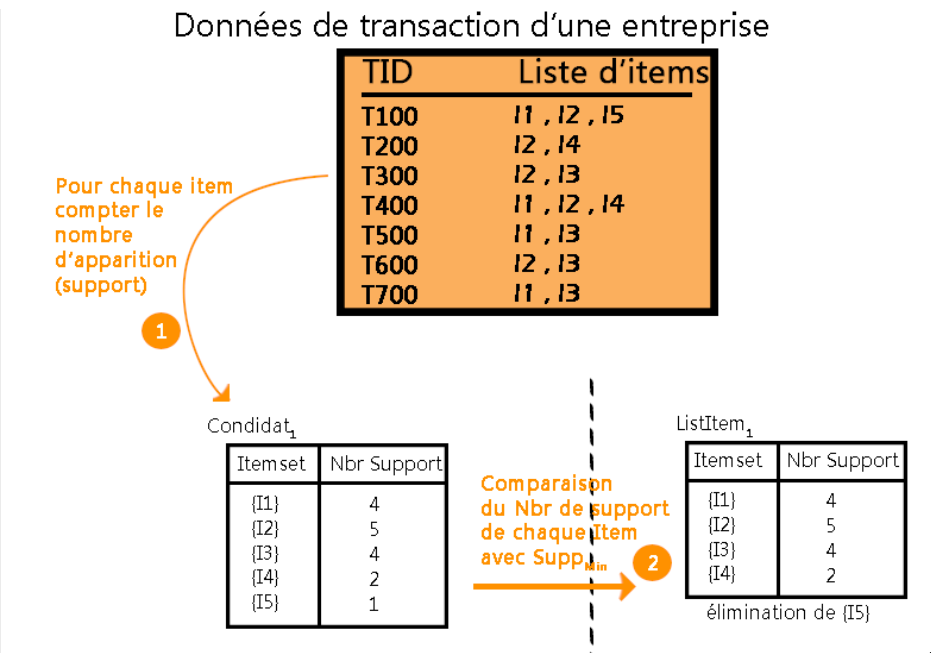
\includegraphics[width=1\textwidth]{image/dm1.PNG}%
\end{center}
\begin{center}
	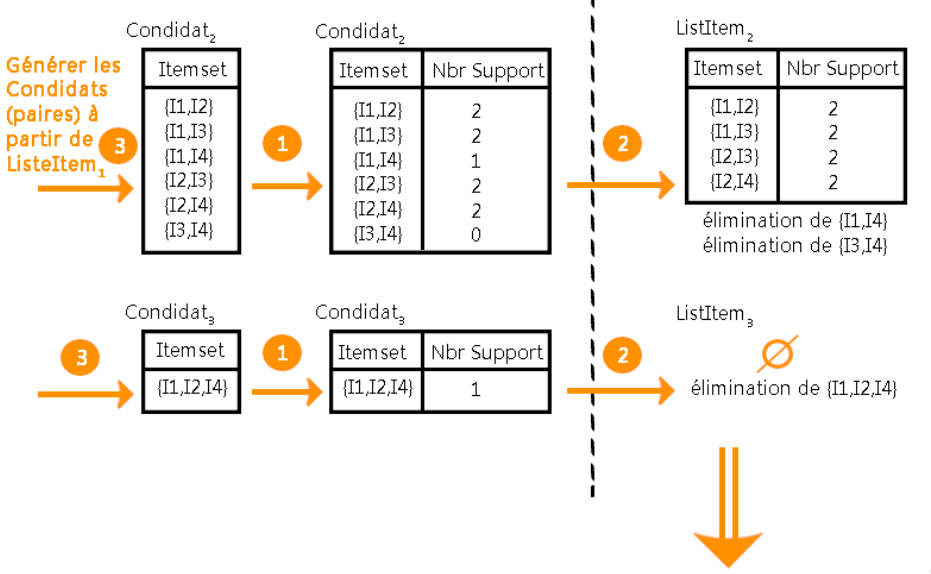
\includegraphics[width=1\textwidth]{image/dm2.PNG}%
\end{center}
\begin{center}
	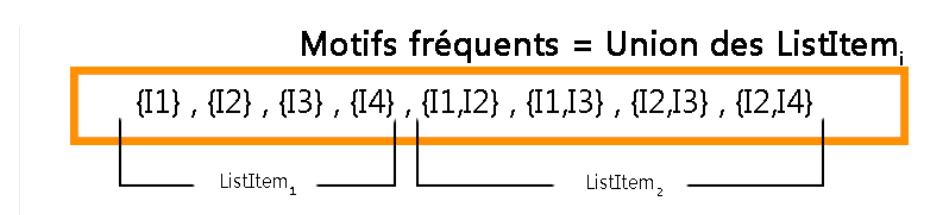
\includegraphics[width=1\textwidth]{image/dm3.PNG}%
	\captionof{figure}{Déroulement de l'algorithme Apriori sur un exemple.}\label{labelname}%
\end{center}



\end{document}